1 & why & 2.1) Why it was created? & its objective/goal (e.g., verify claims, replicability, reusability, a whole new library/framework) & \raisebox{-.5\height}{
\includegraphics[width=0.4\textwidth]{img/likert/priority_why_q1_p2.pdf}}\\\hline
2 & who & 4.2) Who are the authors? & the names of its authors & \raisebox{-.5\height}{
\includegraphics[width=0.4\textwidth]{img/likert/priority_who_q2_p2.pdf}}\\\hline
3 & who & 4.2) Who are the authors? & the contact details of its authors (e.g., email address, ResearchGate, Linkedin, website) & \raisebox{-.5\height}{
\includegraphics[width=0.4\textwidth]{img/likert/priority_who_q2_p4.pdf}}\\\hline
4 & who & 4.1) Who could use it? & be deposited under an explicit open license (e.g., reported in a LICENSE file) & \raisebox{-.5\height}{
\includegraphics[width=0.4\textwidth]{img/likert/priority_who_q1_p1.pdf}}\\\hline
5 & where & 3.3) Where to find related work? & credit to data obtained from other sources (e.g., cited authors, paper, repository) & \raisebox{-.5\height}{
\includegraphics[width=0.4\textwidth]{img/likert/priority_where_q3_p1.pdf}}\\\hline
6 & where & 3.1) Where is it hosted? & is open and public (e.g., GitHub, BitBucket, Zenodo, Figshare) & \raisebox{-.5\height}{
\includegraphics[width=0.4\textwidth]{img/likert/priority_where_q1_p1.pdf}}\\\hline
7 & when & 5.1) When did changes happen? & tracked using version control (e.g., GitHub, GitLab, BitBucket) & \raisebox{-.5\height}{
\includegraphics[width=0.4\textwidth]{img/likert/priority_when_q1_p1.pdf}}\\\hline
8 & what & 1.3) What concepts and technologies underpin the artifact? & the modeling languages used to develop it (e.g., UML, xtUML, SysML, BPMN) & \raisebox{-.5\height}{
\includegraphics[width=0.4\textwidth]{img/likert/priority_what_q3_p2.pdf}}\\\hline
9 & what & 1.3) What concepts and technologies underpin the artifact? & the libraries, dependencies, and frameworks used to develop it and their respective versions (e.g., Eclipse release) & \raisebox{-.5\height}{
\includegraphics[width=0.4\textwidth]{img/likert/priority_what_q3_p6.pdf}}\\\hline
10 & what & 1.2) What does it have? & everything required for replications (i.e., complete) & \raisebox{-.5\height}{
\includegraphics[width=0.4\textwidth]{img/likert/priority_what_q2_p2.pdf}}\\\hline
11 & what & 1.1) What is it all about? & the context of its development (e.g., domain, problem, project) & \raisebox{-.5\height}{
\includegraphics[width=0.4\textwidth]{img/likert/priority_what_q1_p2.pdf}}\\\hline
12 & what & 1.1) What is it all about? & its name & \raisebox{-.5\height}{
\includegraphics[width=0.4\textwidth]{img/likert/priority_what_q1_p1.pdf}}\\\hline
13 & what & 1.1) What is it all about? & its main functionalities supported (e.g., modelling language, code generation, model analysis) & \raisebox{-.5\height}{
\includegraphics[width=0.4\textwidth]{img/likert/priority_what_q1_p3.pdf}}\\\hline
14 & howmuch & 7.1) How many resources does it need? & The artifact shall indicate the system and environment where it was successfully evaluated (e.g., OS, CPU, RAM, GPU, Disk) & \raisebox{-.5\height}{
\includegraphics[width=0.4\textwidth]{img/likert/priority_howmuch_q1_p1.pdf}}\\\hline
15 & how & 6.5) How to run the analysis of results? & The artifact shall provide a clear description of the measurement procedures and metrics used in the paper & \raisebox{-.5\height}{
\includegraphics[width=0.4\textwidth]{img/likert/priority_how_q5_p3.pdf}}\\\hline
16 & how & 6.4) How to replicate the experiment? & The artifact shall provide instructions for manual/automated replication of the complete (or at least a subset) experiment as in the paper (e.g., bash, python, R script) & \raisebox{-.5\height}{
\includegraphics[width=0.4\textwidth]{img/likert/priority_how_q4_p3.pdf}}\\\hline
17 & how & 6.4) How to replicate the experiment? & The artifact shall include the complete set of test models considered & \raisebox{-.5\height}{
\includegraphics[width=0.4\textwidth]{img/likert/priority_how_q4_p1.pdf}}\\\hline
18 & how & 6.3) How to get started? & The artifact shall include step-by-step instructions for running it (e.g., README, PDF) & \raisebox{-.5\height}{
\includegraphics[width=0.4\textwidth]{img/likert/priority_how_q3_p3.pdf}}\\\hline
19 & how & 6.3) How to get started? & The artifact shall include instructions for running it on minimal test data (e.g., quick run, smoke testing) & \raisebox{-.5\height}{
\includegraphics[width=0.4\textwidth]{img/likert/priority_how_q3_p1.pdf}}\\\hline
20 & how & 6.2) How to set up a running environment? & The artifact shall provide instructions to install it & \raisebox{-.5\height}{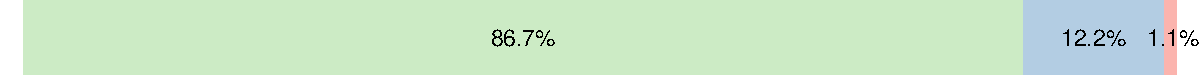
\includegraphics[width=0.4\textwidth]{img/likert/priority_how_q2_p8.pdf}}\\\hline
21 & how & 6.2) How to set up a running environment? & The artifact shall provide instructions for downloading & \raisebox{-.5\height}{
\includegraphics[width=0.4\textwidth]{img/likert/priority_how_q2_p1.pdf}}\\\hline
22 & how & 6.2) How to set up a running environment? & The artifact shall provide a step-by-step tutorial of how to build the source code & \raisebox{-.5\height}{
\includegraphics[width=0.4\textwidth]{img/likert/priority_how_q2_p5.pdf}}\\\hline
23 & how & 6.1) How is it organized? & Files and folders shall have self-explaining names matching content, meaning, and human abstractions (e.g., doc/, src/, results/, src/, bin/) & \raisebox{-.5\height}{
\includegraphics[width=0.4\textwidth]{img/likert/priority_how_q1_p2.pdf}}\\\hline
